\documentclass[11pt]{article}
\usepackage{setspace}
\setstretch{1}
\usepackage[T1]{fontenc}
\usepackage{amsmath,amssymb, amsthm}
\usepackage{graphicx}
\usepackage{bm}
\usepackage[hang, flushmargin]{footmisc}
\usepackage[colorlinks=true]{hyperref}
\usepackage[nameinlink]{cleveref}
\usepackage{footnotebackref}
\usepackage{url}
\usepackage{listings}
\usepackage[most]{tcolorbox}
\usepackage{inconsolata}
\usepackage[papersize={8.5in,11in}, margin=1in]{geometry}
\usepackage{float}
\usepackage{caption}
\usepackage{esint}
\usepackage{url}
\usepackage{enumitem}
\usepackage{subfig}
\usepackage{wasysym}
\newcommand{\ilc}{\texttt}
\usepackage{etoolbox}
\usepackage{algorithm}
% \usepackage{algorithmic}
\usepackage[noend]{algpseudocode}
\usepackage{tikz}
\usetikzlibrary{matrix,positioning,arrows.meta,arrows}
\patchcmd{\thebibliography}{\section*{\refname}}{}{}{}

\makeatletter
\renewcommand{\@seccntformat}[1]{}
\makeatother


\begin{document}



\title{\textbf{EECS 340: Assignment 6}}

\author{Shaochen (Henry) ZHONG, \ilc{sxz517} \\ Yuhui ZHANG, \ilc{yxz2052}}
\date{Due and submitted on 04/20/2020 \\ EECS 340, Dr. Koyut{\"u}rk}
\maketitle

% % % % % % % % % % % % % % % % % % % % % % % % % % % % % % % % % %
% % % % % % % % % % % % % % % % % % % % % % % % % % % % % % % % % %
% % % % % % % % % % % % % % % % % % % % % % % % % % % % % % % % % %
\section{Problem 1}

Hi Grader! Please note the boxes in following diagrams are merely provided for visualization purposes, they are not propertionaly graphed. Thanks.


% % % % % % % % % % % % % % % % % % % % % % % % % % % % % % % % % %
% % % % % % % % % % % % % % % % % % % % % % % % % % % % % % % % % %
\subsection{(a)}

\begin{figure}[H]
    \centering
    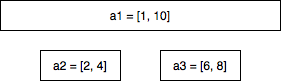
\includegraphics[width=0.4\linewidth]{{fig/fig_1_a.png}}
    \label{fig:1_a}
\end{figure}

\begin{itemize}
    \item Greedy Choice: \ilc{(a1)}
    \item Optimal Choice: \ilc{(a2, a3)}
\end{itemize}

% % % % % % % % % % % % % % % % % % % % % % % % % % % % % % % % % %
% % % % % % % % % % % % % % % % % % % % % % % % % % % % % % % % % %
\subsection{(b)}

\begin{figure}[H]
    \centering
    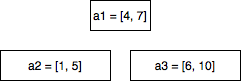
\includegraphics[width=0.4\linewidth]{{fig/fig_1_b.png}}
    \label{fig:1_a}
\end{figure}

\begin{itemize}
    \item Greedy Choice: \ilc{(a1)}
    \item Optimal Choice: \ilc{(a2, a3)}
\end{itemize}

% % % % % % % % % % % % % % % % % % % % % % % % % % % % % % % % % %
% % % % % % % % % % % % % % % % % % % % % % % % % % % % % % % % % %
\subsection{(c)}


\begin{figure}[H]
    \centering
    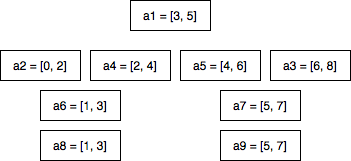
\includegraphics[width=0.4\linewidth]{{fig/fig_1_c.png}}
    \label{fig:1_a}
\end{figure}

\begin{itemize}
    \item Greedy Choice: \ilc{(a1)}
    \item Optimal Choice: Any combination between one of \ilc{\{a2, a4, a5, a6\}} and one of \ilc{\{a3, a7, a8, a9\}}.
\end{itemize}

% % % % % % % % % % % % % % % % % % % % % % % % % % % % % % % % % %
% % % % % % % % % % % % % % % % % % % % % % % % % % % % % % % % % %
% % % % % % % % % % % % % % % % % % % % % % % % % % % % % % % % % %
\section{Problem 2}




% % % % % % % % % % % % % % % % % % % % % % % % % % % % % % % % % %
% % % % % % % % % % % % % % % % % % % % % % % % % % % % % % % % % %
% % % % % % % % % % % % % % % % % % % % % % % % % % % % % % % % % %
\section{Problem 3}

% % % % % % % % % % % % % % % % % % % % % % % % % % % % % % % % % %
% % % % % % % % % % % % % % % % % % % % % % % % % % % % % % % % % %
\subsection{(a)}

Assume we have a set of coins with value of $\{\$1, \$5, \$8\}$ and we are looking to exchange $n = 20$.\newline

The greedy chioce will lead to a solution $\{2 \times \$8, 4 \times \$1\}$ for a totle of $6$ coins, however the optimal solution should be $\{4 \times \$5\}$ for total of $4$ coins. $4 < 6$ and thus disprove the greedy choice property.

% % % % % % % % % % % % % % % % % % % % % % % % % % % % % % % % % %
% % % % % % % % % % % % % % % % % % % % % % % % % % % % % % % % % %
\subsection{(b)}

Assuming we have an optimal solution of $S = <x_o, x_1, x_2, ..., x_k>$, where each $x_i$ respectively represent the amount of $c_i$ coin in the avalivable coin denominations $\{c_1, c_2, ..., c_k\}$ for $1 \leq i \leq k$.

We may observe that there must be $x_i < \frac{c_{i+1}}{c_i}$ for all $1 \leq i \leq k$; as otherwise we may have solution $S' = <x'_o, x'_1, x'_2, ..., x'_k>$ with $x'_i = x_i - \frac{c_{i+1}}{c_i}$ and $x'_{i+1} = x_{i+1} + 1$\footnote{This increment might have to be repeatedly done until the condition of $x_i < \frac{c_{i+1}}{c_i}$ is reached.}. Due to the fact that $\frac{c_{i+1}}{c_i}$ is at least $2$, $S'$ will be a more optimal solution than $S'$ and therefore voids the optimal assumption of $S$. Thus, the property of $x_i < \frac{c_{i+1}}{c_i}$ must be held in the optimal solution.

Knowing this property, we may safely reach the optimal solution $S$ by keep greedily picking the coins with largest $c$ value possible ($c_{\text{max}} \leq n$). Since if we don't pick -- or don't pick the largest amount possible of -- $c_i$ coin(s) at one point, we will have to pick more $c_j$ coins after (for $1 \leq j < i \leq n$), and that will result in a less optimal solution.

% \section{References}
%
% \nocite{*}
% \raggedright
% \bibliography{references.bib}
% \bibliographystyle{plain}


\end{document}